\section{PopQA: The Positive Stable-Recurrence Regime}

PopQA is the paper's clean positive regime. It isolates a recurring-memory setting where support can be reused safely and contradiction risk is low. In that setting, delayed utility helps.

\begin{table}[h]
\centering
\small
\begin{tabular}{llrrrrr}
\toprule
Model & Policy & Quality & 95\% CI & Retrieve & Read & Write \\
\midrule
FLAN-T5 Base & Retrieval only & 0.290 & [0.290, 0.290] & 100.0 & 0.0 & 0.0 \\
FLAN-T5 Base & Retrieve gate & 0.290 & [0.290, 0.290] & 100.0 & 0.0 & 0.0 \\
FLAN-T5 Base & Full router & 0.290 & [0.290, 0.290] & 72.2 & 75.0 & 49.8 \\
FLAN-T5 Base & Calibrated router & 0.290 & [0.290, 0.290] & 72.2 & 75.0 & 49.8 \\
FLAN-T5 Base & Router without delayed utility & 0.090 & [0.090, 0.090] & 36.0 & 15.0 & 14.0 \\
\bottomrule
\end{tabular}

\caption{Official PopQA recurring-memory result. The full router matches retrieval quality while reducing retrieval calls through memory reuse.}
\label{tab:popqa-main}
\end{table}

\begin{figure}[h]
\centering
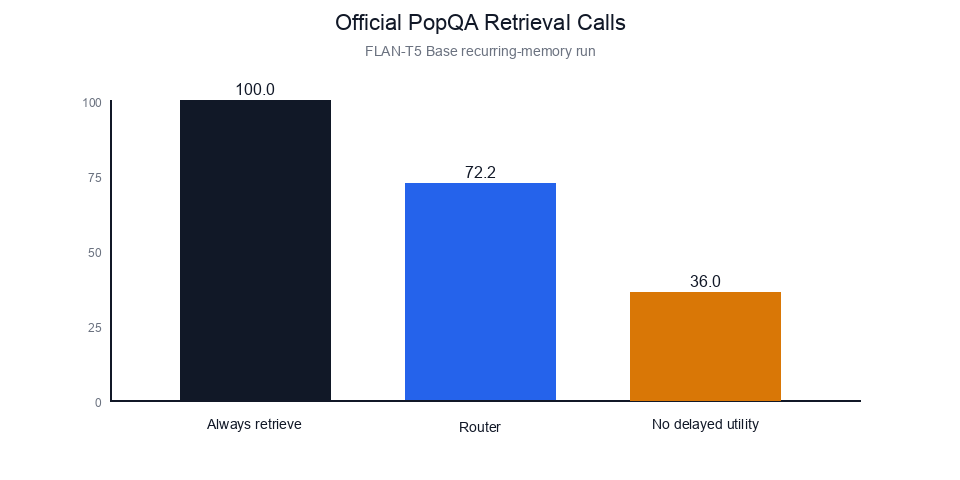
\includegraphics[width=0.82\linewidth]{../shared/generated/word_assets/popqa_retrieval_calls_reduction.png}
\caption{Official PopQA retrieval reduction. The router preserves answer quality while replacing a substantial fraction of repeated retrieval with memory reads and writes.}
\label{fig:popqa-reduction}
\end{figure}

The official FLAN-T5-Base run is straightforward. Retrieval-only, the retrieve gate, the full router, and the calibrated router all achieve 0.290 quality. The full router and calibrated router reduce retrieval calls from 100.0 to 72.2 while issuing 75.0 memory reads and 49.8 memory writes. In contrast, \texttt{router\_no\_v\_future} drops to 0.090 quality with much weaker memory use. The paired sign tests sharpen the same story: the full router is tied with retrieval (\(p = 1.0\)), while suppressing delayed utility is significantly worse (\(p = 1.58 \times 10^{-30}\)).

This is the paper's strongest direct evidence that future value changes the preferred policy in stable recurring-memory settings. The positive claim should therefore be read narrowly but confidently: delayed utility is useful when support is stable enough to be written once and reused later without incurring contradiction risk.
